%%%%%%%%%%%%%%%%%%%%%%%%%%%%%%%%%%%%%%%%%%%%%%
% To select a journal, use its code for the 
% journal= option in the \documentclass command.
% The journal codes for this template are:
% 
% Annals of Actuarial Science: aas
% British Journal of Political Science: jps
% Network Science: nws
% Political Analysis: pla
% Political Science Research and Methods: ram
% Evolutionary Human Sciences: ehs
% Natural Language Processing: nlp
%%%%%%%%%%%%%%%%%%%%%%%%%%%%%%%%%%%%%%%%%%%%%%
\documentclass[
  journal=largetwo,
  manuscript=article-type,
  year=2026,
  volume=37,
]{cup-journal}

\usepackage{amsmath}
\usepackage[nopatch]{microtype}
\usepackage{booktabs}
\usepackage{parskip} 
\usepackage{enumitem}
\setlist[itemize]{left=1em}
\usepackage{titlesec}
% Espacio después de los títulos
\titlespacing*{\section}{0pt}{0.6\baselineskip}{0.6\baselineskip}
\titlespacing*{\subsection}{0pt}{0.5\baselineskip}{0.5\baselineskip}
\titlespacing*{\subsubsection}{0pt}{0.4\baselineskip}{0.4\baselineskip}

\title{Visión Artificial - Actividad 2: Exploración de filtros espaciales y morfológicos en escenarios reales}

\author{Orejón Blázquez, Álvaro}
\affiliation{Estudiantes, Universidad Internacional de La Rioja}
\email[Orejón Blázquez, Álvaro]{alvaro.orejonbl0659@comunidadunir.net}

\author{Lopez Chamarro, Pau}
\affiliation{Estudiantes, Universidad Internacional de La Rioja}
\email[Lopez Chamarro, Pau]{pau.chamarro455@comunidadunir.net}

\author{Iglesias Traviesa, Nuria}
\affiliation{Estudiantes, Universidad Internacional de La Rioja}
\email[Iglesias Traviesa, Nuria]{nuria.iglesias660@comunidadunir.net}

\author{Prieto Bailo, León Enrique}
\affiliation{Estudiantes, Universidad Internacional de La Rioja}
\email[Prieto Bailo, León Enrique]{leonenrique.pri7080@comunidadunir.net}
% \author{T. Author}
% \affiliation{Second Division, Organization, City, Pincode, State, Country}

% \author{F.T. Author}
% \affiliation{Fourth Division, Organization, City, Pincode, State, Country}

\addbibresource{bibliography.bib}

\keywords{visión artificial, procesamiento digital de imágenes, filtros espaciales, operaciones morfológicas, filtros de suavizado, detección de bordes}

\begin{document}

\begin{abstract}
Este trabajo explora el comportamiento de distintos \textit{filtros espaciales} y \textit{operaciones morfológicas} aplicados sobre imágenes reales de distintos ámbitos (escenarios médico, industrial y satelital/ambiental). 
El objetivo principal es comparar cómo cada técnica modifica la información visual, la preservación de estructuras relevantes y la interpretabilidad del contenido. 
En concreto, se analizan su impacto tanto de forma cualitativa (inspección visual de la pérdida de detalle, eliminación de artefactos y cambios en contornos) como cuantitativa mediante métricas como PSNR, SSIM, entropía y un índice de preservación de bordes (EPI). 
Los resultados obtenidos muestran que la eficacia de cada transformación depende fuertemente del contexto: los filtros de suavizado tienden a reducir ruido y detalle fino a costa de degradar bordes, mientras que las operaciones morfológicas permiten regular la conectividad y la geometría de las regiones de interés con cambios controlados en la estructura global.
El estudio pone de manifiesto que no existe un filtro universalmente óptimo y que la selección de parámetros debe ajustarse al tipo de imagen y al objetivo de análisis. 
\end{abstract}

\section{Introducción}
\label{sec:intro}

El procesamiento digital de imágenes es una disciplina fundamental que permite mejorar, analizar e interpretar entornos reales. En campos donde se utilizan imágenes digitales, como la industria y la medicina, la aplicación de filtros
espaciales y morfológicos se ha convertido en una herramienta esencial para optimizar la calidad de las imágenes y extraer información relevante. Esto se debe a que las imágenes capturadas suelen estar afectadas por ruido, baja resolución y condiciones de iluminación,
lo que dificulta su análisis. La aplicación de estos filtros mejora la calidad visual de las imágenes, facilitando así su análisis y la extracción de información para la toma de decisiones.

Los filtros espaciales actúan modificando la intensidad de los píxeles en función de su vecindad, permitiendo así reducir ruido, suavizar regiones homogéneas y realzar o detectar bordes. Por otra banda, los filtros morfológicos actúan sobre la forma y estructura de los objetos mediante 
operaciones como la erosión, dilatación, apertura o cierre. Estas técnicas permiten eliminar elementos no deseados, separar o unir regiones y mejorar contornos.

Este trabajo presenta un enfoque multitemático que aplica, mediante un pipeline, un conjunto de filtros espaciales y morfológicos sobre imágenes de contextos médico, satelital e industrial. Este proceso permite comparar de forma directa los efectos de cada técnica dependiendo 
de la imagen utilizada. Además, se analiza cómo estas herramientas influyen en la calidad visual, la preservación de estructuras y la interpretabilidad de la información, identificando así las ventajas y limitaciones de cada filtro. De esta manera, se puede afirmar que 
no existe un filtro universalmente óptimo, y que la eficacia de cada técnica depende del contexto y de las características específicas de cada imagen.

\section{Material y métodos}
\label{sec:mat}

\subsection{Software utilizado}
\label{subsec:software}

El desarrollo se llevó a cabo en \textbf{Jupyter Notebook} \parencite{jupyter-notebook-official} (\textbf{Python} \cite{python-official}) ejecutado desde \textbf{Visual Studio Code} \parencite{vscode-official}, mediante librerías ampliamente utilizadas para garantizar una implementación reproducible.
Se decidió el uso de este entorno para disponer en un mismo flujo de trabajo la carga de imágenes, la aplicación de los algoritmos de filtrado y la visualización de los resultados.
El observar las imágenes originales y procesadas de manera consistente facilitó la comparación y nos permitió comprender en profundidad el efecto de cada de las distintas transformaciones aplicadas.

En particular, se empleó \textbf{OpenCV} \parencite{opencv-official} (\texttt{cv2}) para la lectura de imágenes, conversión de color y la implementación de los filtros espaciales y morfológicos, eligiendo esta librería por numerosas razones, entre ellas sus funciones optimizadas para tareas de manipulación de imágenes, como la detección de bordes y la aplicación de diversos filtros.
Las operaciones de apoyo, como preprocesado y postprocesado, se realizaron con la librería \textbf{NumPy} \parencite{numpy-official}, que es fundamental en el manejo de grandes volúmenes de datos, ya que proporciona herramientas para realizar operaciones matemáticas sobre matrices multidimensionales.
Por último, \textbf{Matplotlib} \parencite{matplotlib-official} se utilizó para la generación de figuras y la comparación visual clara y efectiva de los efectos de cada técnica sobre las imágenes.

Para asegurar aún más la reproducibilidad, se tomó la decisión de crear la implementación de forma que los resultados sean replicables bajo las mismas condiciones de ejecución.

\subsection{Selección de imágenes}
\label{sec:imagenes}

Con el objetivo de evaluar el comportamiento de filtros espaciales y operaciones morfológicas en un escenario multitemático, 
se trabajó con un conjunto acotado de imágenes reales seleccionadas de tres ámbitos diferenciados: \textit{industrial}, \textit{médico} y \textit{satelital/ambiental}. 

La selección se realizó siguiendo criterios orientados a maximizar la diversidad, es decir, priorizando ejemplos representativos con propiedades visuales claramente distintas. 
Al aplicar distintos filtros a cada una de las imágenes, se hizo posible la comparación entre las técnicas en condiciones cambiantes.

Estas imágenes fueron extraídas de tres fuentes principales, cada una para un tipo de escenario:
\begin{itemize}
    \item \textbf{Open-i (escenario médico)} \parencite{openi-nlm}. Open-i es un repositorio y motor de búsqueda de imágenes biomédicas mantenido por la \textit{National Library of Medicine}, que nos permitió obtener imágenes relacionadas con la temática biomédica. 
    En esta práctica se empleó para seleccionar radiografías, donde predominan gradientes suaves y estructuras anatómicas con bordes definidos, lo que resulta extremadamente adecuado para analizar la atenuación de ruido mediante suavizado y los detectores de borde.

    \item \textbf{Science Source (escenario industrial)} \parencite{sciencesource}. Science Source es una biblioteca científica con imágenes relacionadas con tecnología, laboratorio e industria. 
    Se utilizó como fuente para seleccionar escenas industriales con patrones geométricos y contornos de alto contraste, idóneas para aplicar el filtrado espacial que afecta al detalle fino y las operaciones morfológicas, que pueden regular este tipo de estructuras.

    \item \textbf{EOSDA LandViewer / Sentinel Playground (escenario satelital y ambiental)} \parencite{eosda-landviewer,sentinel-playground}. Se recurrió a plataformas de exploración ambiental y de imágenes satelitales.
    Estas nos proporcionan imágenes con grandes regiones homogéneas y elementos lineales (carreteras), lo que facilita comparar el comportamiento de los filtros cuando se enfrentan a variaciones de escala y contenido.
\end{itemize}

\subsection{Filtros espaciales}
\label{sec:esp}

Los filtros espaciales son operadores fundamentales en el procesado digital de imágenes y la visión por computador los cuales modifican las intensidades de los pixeles en base a los vecinos locales. A diferencia de otros métodos basados en dominios frecuenciales, el filtro espaciado se realiza en el dominio de la imagen, donde la salida de cada pixel es calculada como una función a partir de los pixeles vecinos definida por una mascara espacial o kernel. 

Formalmente, un filtro espacial puede ser descrito como una función que desliza una pequeña matriz (kernel) sobre la imagen, calculando un nuevo valor de píxel en cada ubicación a través de una operación predefinida. En el caso de los filtros espaciales lineales, esta operación corresponde a una convolución o correlación entre la imagen y el kernel. Los filtros espaciales no lineales, por otro lado, se basan en operaciones no lineales como la selección de mínimos, máximos o medianas dentro de la vecindad de pixeles.

Los filtros espaciales se categorizan habitualmente en función de los objetivos que persiguen. Los filtros de suavizado (o paso bajo) buscan reducir el ruido y pequeñas variaciones de intensidad promediando el valor de los píxeles en la vecindad. Ejemplos típicos incluyen filtros Gaussianos y de media, ampliamente utilizados como paso de preprocesado para mejorar la calidad y robustez de la imagen en análisis posteriores. Por el contrario, filtros como el realce de bordes enfatizan cambios de intensidad locales, resaltando bordes y detalles finos. Estos filtros son particularmente útiles para la extracción de características, detección de objetos y tareas de segmentación.

La efectividad de un filtro espacial depende de varios factores, incluyendo el tamaño y forma del kernel, el tipo de operación aplicada, y las características de la propia imagen. Un kernel excesivamente largo puede suavizar excesivamente estructuras importantes, mientras que un filtro de realce inadecuado puede amplificar ruido e introducir artefactos. Por lo tanto, la selección de filtros espaciales debe ser adaptada cuidadosamente en función de la aplicación y el contexto de la imagen. 

En escenarios prácticos, el filtrado espacial juega un rol crucial en diversos escenarios como la fotografía medica, la inspección industrial, la teledetección, y el análisis de imágenes biológicas. Al mejorar estructuras relevantes y mitigando variaciones indeseadas, los filtros espaciales facilitan la interpretación de información visual y mejoran el rendimiento de los algoritmos de visión por computador.

\subsubsection{Suavizado}
\label{sec:suavizado}

Los filtros de suavizado, también conocidos como filtros paso bajo, son una clase de filtros espaciales cuyo objetivo principal consiste en atenuar variaciones rápidas de intensidad de las imágenes las cuales están normalmente asociadas con ruido y detalles de alta frecuencia. Como resultado, los filtros de suavizado se emplean habitualmente como una de las etapas del preprocesado para la mejora de la calidad y para mejorar la robustez de tareas posteriores como la segmentación, detección de bordes y extracción de características. 

Conceptualmente, los filtros de suavizado funcionan agregando información de intensidad dentro de una vecindad local alrededor de cada pixel. Combinando los valores de la vecindad, se logra la atenuación de cambios de intensidad abruptos y se mantienen los cambios suaves en las regiones. Este proceso, conlleva una reducción de ruido pero introduce inevitablemente un cierto grado de desenfoque, particularmente en las fronteras de los objetos presentes. Consecuentemente, la aplicación del filtro paso-bajo implica un \textit{trade-off} entre la supresión de ruido y la conservación de los bordes. 

Los filtros de suavizado pueden ser clasificados entre lineales y no lineales. Los filtros lineales calculan la salida de cada pixel como la suma ponderada de las intensidades de la vecindad. El filtro mas sencillo es el filtro de media, el cual reemplaza cada pixel con la media aritmética de los pixeles circundantes. Si bien es eficaz para reducir ruido Gaussiano, el filtro de media tiende a difuminar los bordes y las estructuras finas. El filtro Gaussiano representa representa una aproximación mas refinada, en la cual los pesos siguen una distribución Gaussiana centrada en el pixel de interés. Este esquema de ponderación enfatiza los pixeles mas cercanos y resulta en un filtrado mas suave y natural, a la vez que ofrece un mejor control sobre el grado de suavizado. 

Los filtros de suavizado no lineales no se basan en operaciones de promediado, sino que aplican transformaciones basadas en estadísticas de orden o reglas. El filtro de mediana es una de las técnicas de suavizado no lineal mas utilizadas. Sustituye cada pixel con el valor de la mediana de las intensidades de la vecindad, haciéndolo particularmente efectivo en la supresión de ruido impulsivo, como el sal y pimienta. Otra ventaja importante de los filtros de media es su habilidad de preservar ejes y fronteras mas efectivamente que los filtros de media. 

El rendimiento de los filtros de suavizado está muy influenciado por el tamaño y forma del kernel, así como las características de ruido presentes en la imagen. Kernels mas pequeños proveen de reducción de ruido limitada a la vez que preservan bien el detalle, mientras que kernels mas grandes generan efectos de suavizado mas fuertes a cambio de la perdida de información estructural. Por lo tanto, la selección del filtro y del tamaño del kernel apropiado debe ser adaptado a la aplicación especifica y el contexto que presenta la imagen. 

\subsubsection{Realce de bordes}
\label{sec:rb}

El realce y la detección de bordes constituyen una de las etapas fundamentales en el procesamiento digital de imágenes y en los sistemas de visión artificial. Los bordes representan discontinuidades significativas en la intensidad de una imagen y suelen corresponder a límites entre objetos, cambios de material o variaciones abruptas de iluminación. La correcta identificación y realce de estos bordes facilita tareas posteriores como la segmentación, el reconocimiento de objetos y la extracción de características \cite{DataImageProcessing}.

Desde un punto de vista matemático, una imagen digital puede considerarse como una función bidimensional de intensidad $f(x, y)$. Un borde se define como una región donde dicha función presenta un cambio brusco, lo que se traduce en:
\begin{itemize}
    \item Valores elevados del gradiente (priemera derivada).
    \item O bien cruces por cero en la segunda derivada.
\end{itemize}
Por este motivo, la mayoría de los filtros de realce de bordes se basan en aproximaciones discretas de derivadas espaciales \cite{Szeliski}.

A continuación se describen los filtros espaciales más comunes utilizados para la detección de estructuras de borde en una imagen.

El operador Roberts emplea máscaras de tamaño $2\times2$ (Figura~\ref{fig:robert_mask}) y está orientado a la detección de bordes diagonales. Debido al reducido tamaño de sus máscaras, es especialmente sensible al ruido, por lo que su uso se limita principalmente a fines didácticos o a imágenes con bajo nivel de ruido.

\begin{figure}[H]
    \centering
    \includegraphics[width=0.5\textwidth]{images/roberts-mask.png}
    \caption{Máscara Operador Roberts}
    \label{fig:robert_mask}
\end{figure}

El operador Sobel aproxima el gradiente de la imagen mediante dos máscaras convolucionales de tamaño $3\times3$ (Figura~\ref{fig:sobel_mask}), orientadas en las direcciones horizontal y vertical. Estas máscaras incorporan un ligero suavizado al ponderar el píxel central, lo que reduce parcialmente la sensibilidad al ruido en comparación con otros operadores de gradiente más simples.

\begin{figure}[H]
    \centering
    \includegraphics[width=0.6\textwidth]{images/sobel-mask.png}
    \caption{Máscara Operador Sobel}
    \label{fig:sobel_mask}
\end{figure}

El operador Prewitt es conceptualmente similar al operador Sobel, ya que utiliza máscaras de tamaño $3\times3$ (Figura~\ref{fig:prewitt_mask}) y permite estimar el gradiente en las direcciones horizontal y vertical. No obstante, emplea coeficientes uniformes en sus máscaras, lo que lo hace ligeramente menos preciso en la estimación del gradiente y algo más sensible al ruido.

\begin{figure}[H]
    \centering
    \includegraphics[width=0.5\textwidth]{images/prewitt-mask.png}
    \caption{Máscara Operador Prewitt}
    \label{fig:prewitt_mask}
\end{figure}

El detector de Canny es considerado uno de los métodos más completos y robustos para la detección de bordes. Su funcionamiento se basa en una secuencia de etapas bien definidas: suavizado Gaussiano para la reducción del ruido, cálculo del gradiente, supresión de no-máximos con el objetivo de obtener bordes finos y bien localizados, y finalmente una umbralización con histéresis para eliminar respuestas débiles no conectadas con bordes significativos.

\subsection{Filtros morfológicos}
\label{sec:morf}

\subsubsection{Dilatación}
\label{sec:Dilatacion}

La dilatación es uno de los operadores esenciales en la morfología matemática y su principal función es expandir las regiones de una imagen binaria, por lo que potencia las zonas de contornos y amplía los objetos presentes \parencite{Serra1982IAMM}.

Matemáticamente, la dilatación se puede expresar como la expansión de la imagen original \( A \) con respecto a un elemento estructural \( B \), de forma que la imagen resultante incrementa el tamaño de los objetos originales \parencite{Haralick1987MM}.
\[
A \oplus B = \bigcap_{b \in B} A_b
\]

El efecto de la dilatación en una imagen depende directamente de la forma y tamaño del elemento estructural utilizado. 
Este elemento, que puede ser un cuadrado, círculo o cualquier otra forma, define el área sobre la cual se realiza la expansión.
La operación se aplica píxel a píxel sobre toda la imagen, comprobando la relación entre el elemento estructural \( B \) y la imagen original \( A \).
Cuando el elemento estructural entra en contacto con el objeto de la imagen, este se dilata en las áreas de solapamiento. 

Se utiliza principalmente para fusionar elementos cercanos, como en la reconstrucción de objetos que fueron segmentados incorrectamente o en el relleno de huecos en una imagen. 
Sin embargo, un efecto importante de la dilatación es que no conserva la forma original del objeto, lo que puede ser útil o perjudicial dependiendo del contexto de la segmentación.

Esta técnica es particularmente útil en escenarios con bajo contraste o cuando los valores de intensidad están concentrados en un rango reducido, como en las imágenes de los escenarios médico y satelital de nuestro dataset. 
Por ejemplo, en las radiografías médicas, la dilatación ayuda a fusionar fragmentos pequeños de estructuras anatómicas, como los huesos o lesiones, que se encuentran parcialmente segmentados o separados debido a la falta de contraste. 
En las imágenes satelitales, la dilatación puede mejorar la visibilidad y conectividad de áreas de interés dispersas, como campos agrícolas o cuerpos de agua.

\subsubsection{Erosión}
\label{sec:erosion}

La erosión es un operador morfológico que aunque lo parezca, no se puede considerar la inversa a la dilatación. Su principal objetivo es reducir el tamaño de los objetos en una imagen, eliminando los detalles y reduciendo los contornos \parencite{Soille2003MIA}. 

Este operador es útil para eliminar pequeños objetos o detalles no deseados en una imagen segmentada.
En el caso de las imágenes médicas, como las radiografías, la erosión puede ayudar a eliminar ruido que permanece tras la segmentación, haciendo que los objetos de interés, como huesos o lesiones, sean más claros y fáciles de analizar. 
En las imágenes satelitales, la erosión es útil cuando se realiza la segmentación de grandes áreas de terreno, como campos agrícolas o zonas urbanas, ya que al simplificar las formas permite una mejor definición de las grandes estructuras como carreteras o edificios.

Matemáticamente, la erosión se puede expresar como la reducción de la imagen original \( A \) con respecto a un elemento estructural \( B \), de forma que la imagen resultante disminuye el tamaño de los objetos originales.
\[
A \ominus B = \bigcup_{b \in B} A_b
\]

La erosión funciona de manera similar a la dilatación, pero en lugar de expandir los objetos, elimina los detalles exteriores. 
El elemento estructural en este caso define el área sobre la cual se realiza la reducción. 
Cuando este se encuentra completamente contenido dentro del objeto de la imagen, la imagen resultante conserva el área de solapamiento, pero elimina los detalles exteriores, reduciendo el tamaño de los objetos.

El resultado de la erosión es que los objetos tienden a desaparecer parcialmente, especialmente aquellos que tienen bordes débiles o que no coinciden en su totalidad con el elemento estructural. 
A diferencia de la dilatación, la erosión conserva menos detalles de la imagen original, lo que puede ser útil para acentuar la forma central de un objeto, facilitando tareas como la detección de bordes.
Sin embargo, la erosión también modifica la forma original del objeto, a menudo eliminando detalles importantes si no se utiliza con precaución.

\subsubsection{Apertura}
\label{sec:ap}

La apertura es una operación morfológica que combina de forma secuencial una erosión seguida de una dilatación, utilizando el mismo elemento estructurante en ambas etapas. En la primera fase, la erosión reduce las regiones brillantes de la imagen y elimina 
pequeñas estructuras o detalles no deseados que no cumplen con el tamaño del elemento estructurante. Esto permite eliminar ruido o irregularidades sin afectar a los objetos principales de la imagen.

A continuación, la dilatación restaura parcialmente el tamaño de los objetos que han sobrevivido a la erosión, manteniendo su forma y sus contornos originales. De esta manera, la operación de apertura suaviza los bordes de los objetos principales 
mientras elimina los elementos de menor tamaño, modificando la estructura de la imagen de forma controlada.

El proceso de apertura actúa principalmente sobre elementos cuya dimensión es menor que la del elemento estructurante, afectando sobre todo a pequeños detalles o uniones entre objetos. El objetivo de esta técnica es obtener imágenes con estructuras más 
limpias y contornos más definidos, facilitando la interpretación y análisis de los objetos presentes en la imagen.

\subsubsection{Cierre}
\label{sec:cierre}

El cierre es una operación morfológica que combina de manera secuencial una dilatación seguida de una erosión, utilizando el mismo elemento estructurante en ambas etapas. En la primera fase, la dilatación expande las regiones brillantes de la imagen, 
rellenando pequeñas separaciones y conectando objetos cercanos que podrían estar ligeramente separados.

A continuación, la erosión reduce parcialmente el tamaño de los objetos que fueron ampliados durante la dilatación, restaurando sus formas originales y manteniendo las conexiones establecidas entre ellos. De esta manera, el cierre permite suavizar los bordes de 
los objetos principales, rellenar huecos y unificar regiones.

El proceso de cierre actúa principalmente sobre elementos más pequeños que el elemento estructurante, afectando a huecos en la imagen mientras conserva la geometría general de los objetos de mayor tamaño. El objetivo de esta técnica es obtener imágenes más uniformes 
y continuas, facilitando la interpretación y el análisis de las estructuras presentes.

\section{Resultados y métricas}
\label{sec:result}

En esta sección se presentan los resultados obtenidos tras la aplicación de los distintos filtros espaciales y morfológicos sobre el conjunto de imágenes seleccionadas. El objetivo principal de este apartado es mostrar de manera clara el efecto que cada técnica
produce a la imagen original. Esto nos permite observar cómo los diferentes filtros modifican la información y la estructura de las imágenes en función de sus características específicas.

Para facilitar la interpretación, los resultados se organizan en dos grandes bloques: \textit{filtros espaciales} y \textit{filtros morfológicos}. Dentro de cada bloque se analiza de forma individual las disitntas técnicas aplicadas. Para cada subtécnica se muestran
tres imágenes representativas, una de cada escenarios : \textit{médico}, \textit{industrial} y \textit{satelital/ambiental}, con el objetivo de ilustrar de manera directa el efecto de cada filtro en contextos variados sobre la imagen original. Además, se incluyen
métricas propias que permiten cuantificar el impacto de cada filtro en términos de calidad visual y preservación de estructuras relevantes.

Este enfoque permite exponer los resultados de manera sistemática, destacando los efectos de cada filtro de forma independiente. De este modo, se proporciona una visión completa tanto cualitativa como cuantitativa del impacto de los filtros aplicados sobre las imágenes 
seleccionadas.

\subsection{Filtros Espaciales}
\label{sec:filtros_esp}
\subsubsection{Suavizado}

En esta sección se presenta la aplicación del filtro de suavizado sobre imágenes seleccionadas de un dataset de Open-I y Science Source. Aunque las imágenes empleadas no contienen altos niveles de ruido u otros efectos como sal y pimienta, donde este filtro destaca particularmente, la aplicación de esta transformación a las imágenes seleccionadas nos permite estudiar su impacto sobre las mismas. 

Se contemplan dos imágenes; para la primera (4800 x 4800 px) se emplea un tamaño de kernel de 25, mientras que para la segunda (512 x 512 px) se utiliza un tamaño de 7. Esta magnitud varía siempre en función del tamaño de la imagen con la que se esté trabajando, del nivel de detalle que se quiera preservar y de la efectividad en la supresión del ruido presente en la imagen. 

Se decide aplicar esta técnica sobre un escenario industrial, ya que posee una gran cantidad de bordes. El objetivo de esta transformación es observar cómo el filtro afecta a la componente estructural de la imagen. Asimismo, se decide aplicarla sobre una radiografía humana, con el fin de analizar la capacidad de eliminar detalles menos relevantes y centrar la imagen en estructuras de mayor tamaño. En este caso, se emplean y comparan filtros gaussianos y de media. 

\begin{figure}[h!]
\centering
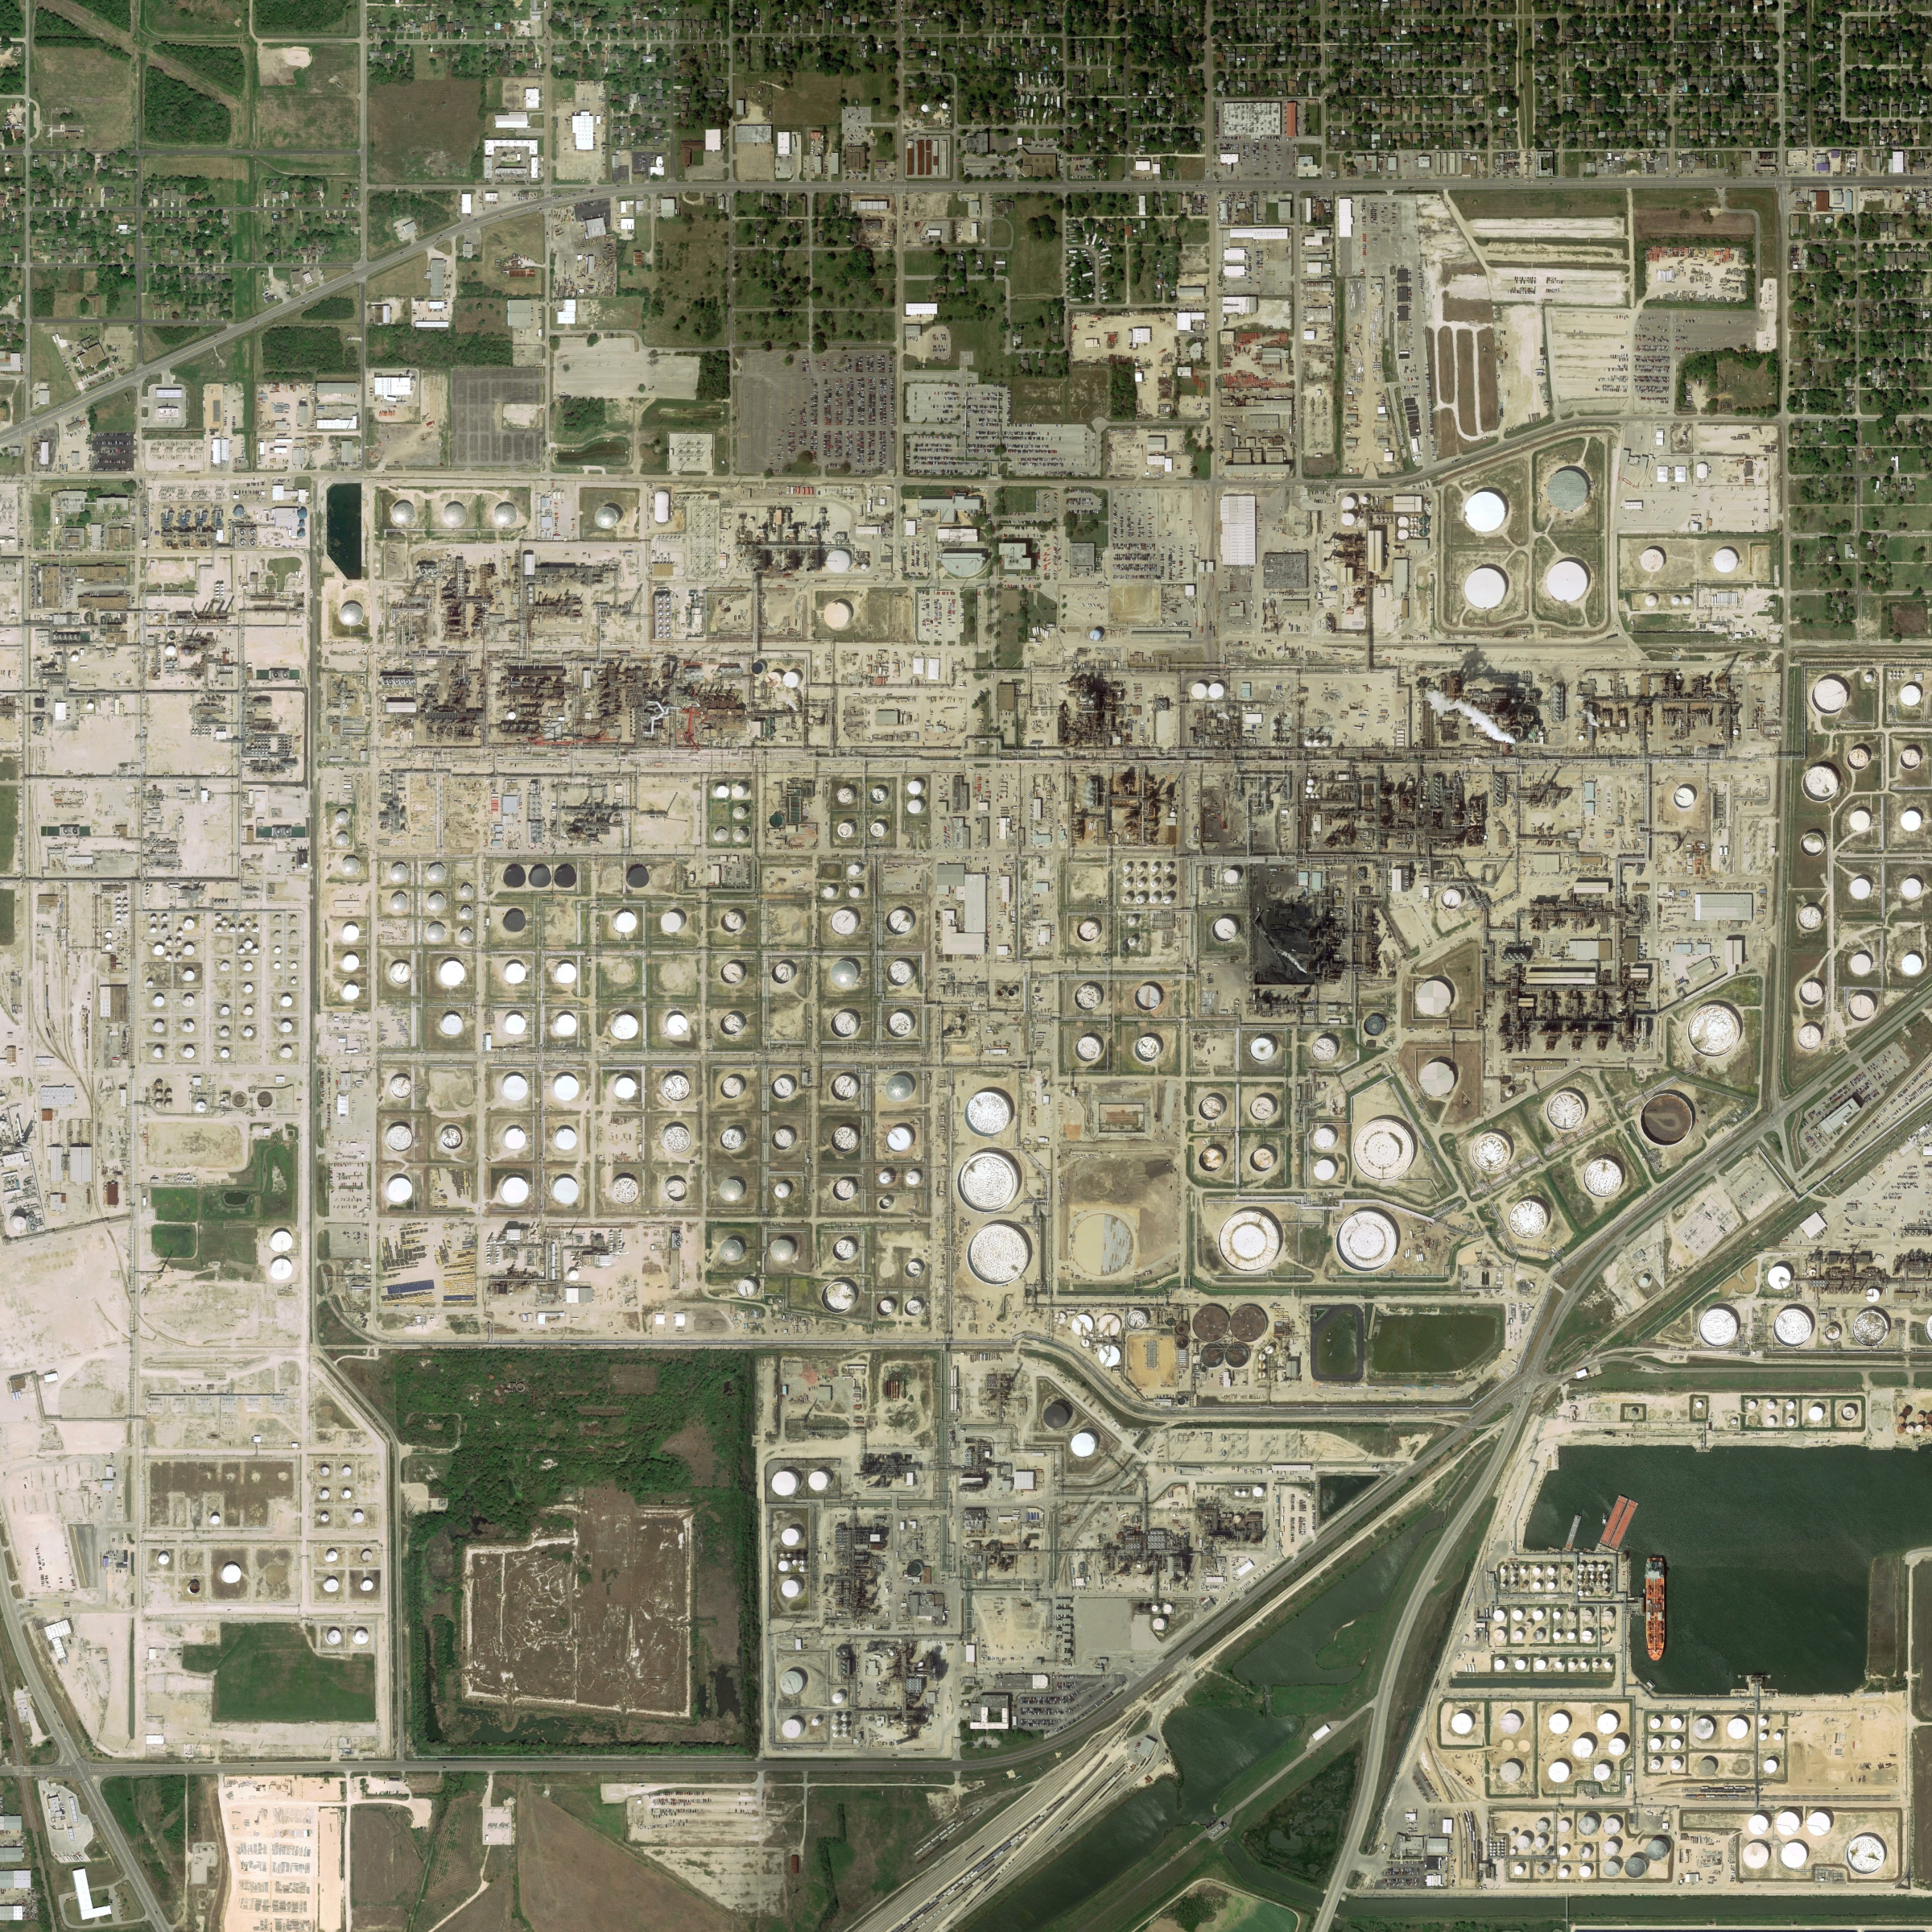
\includegraphics[width=0.25\textwidth]{images/smooth-filter/img1_original.png}
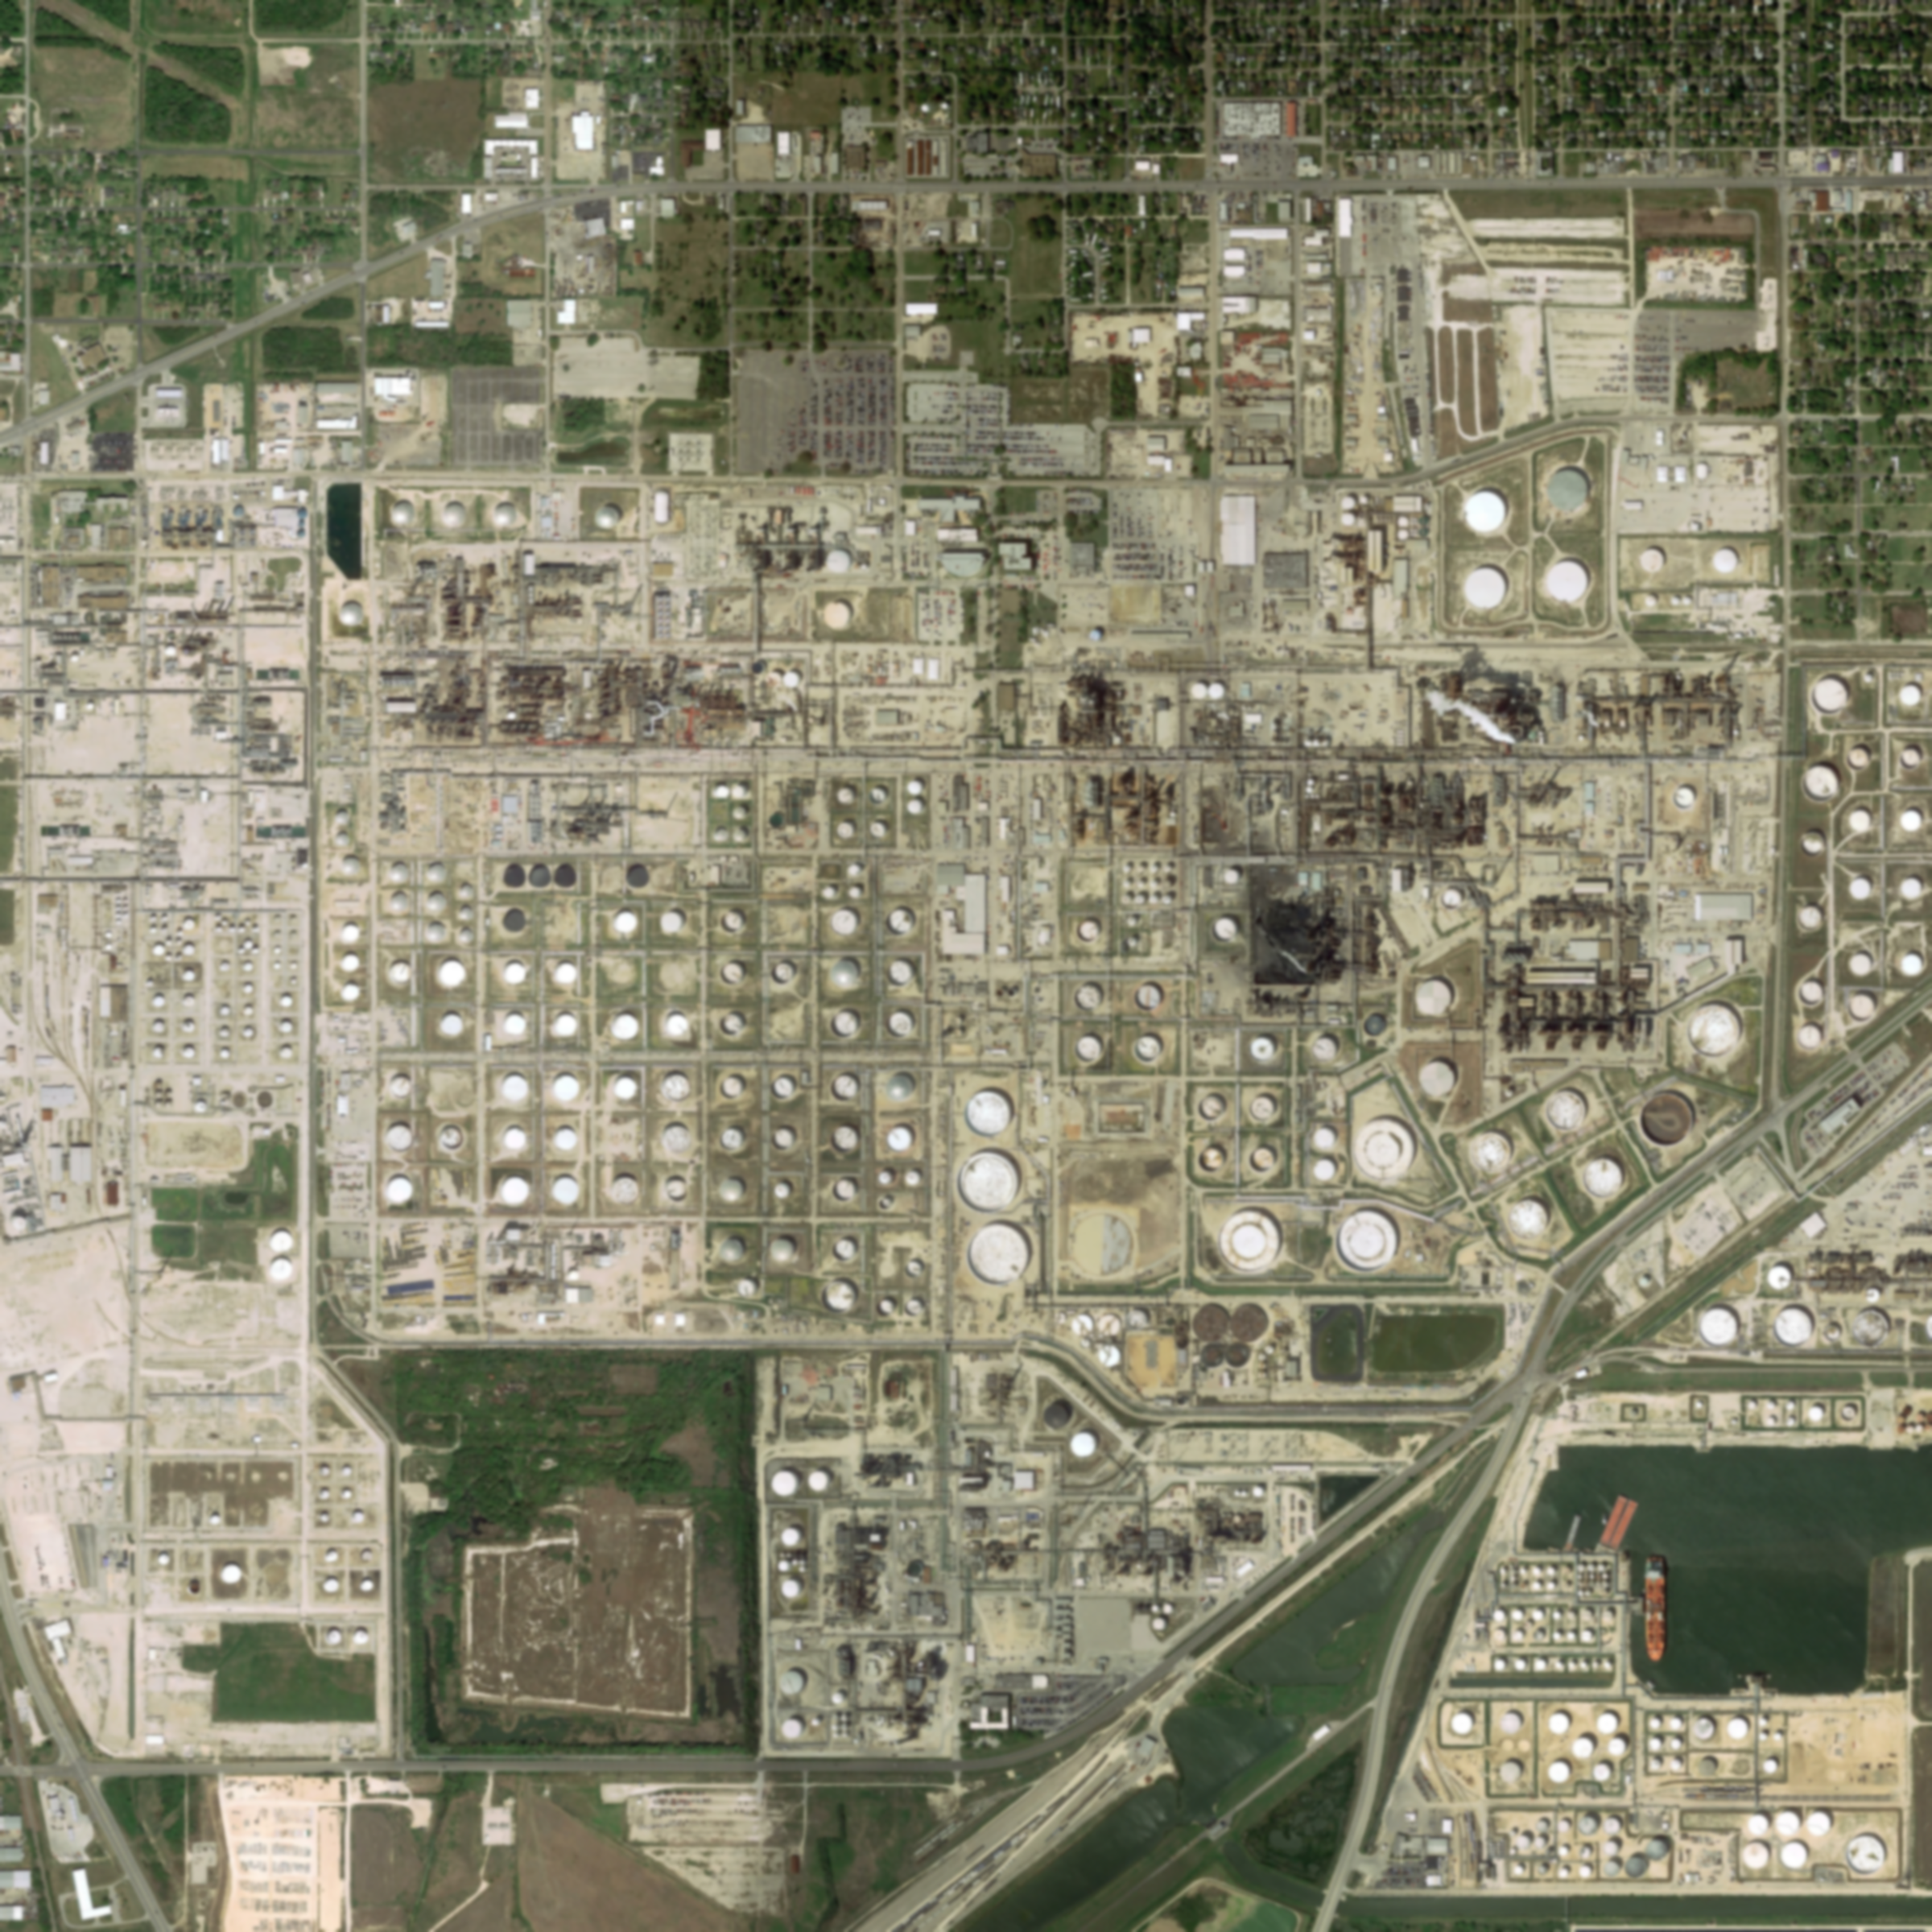
\includegraphics[width=0.25\textwidth]{images/smooth-filter/img1_gaussian.png}
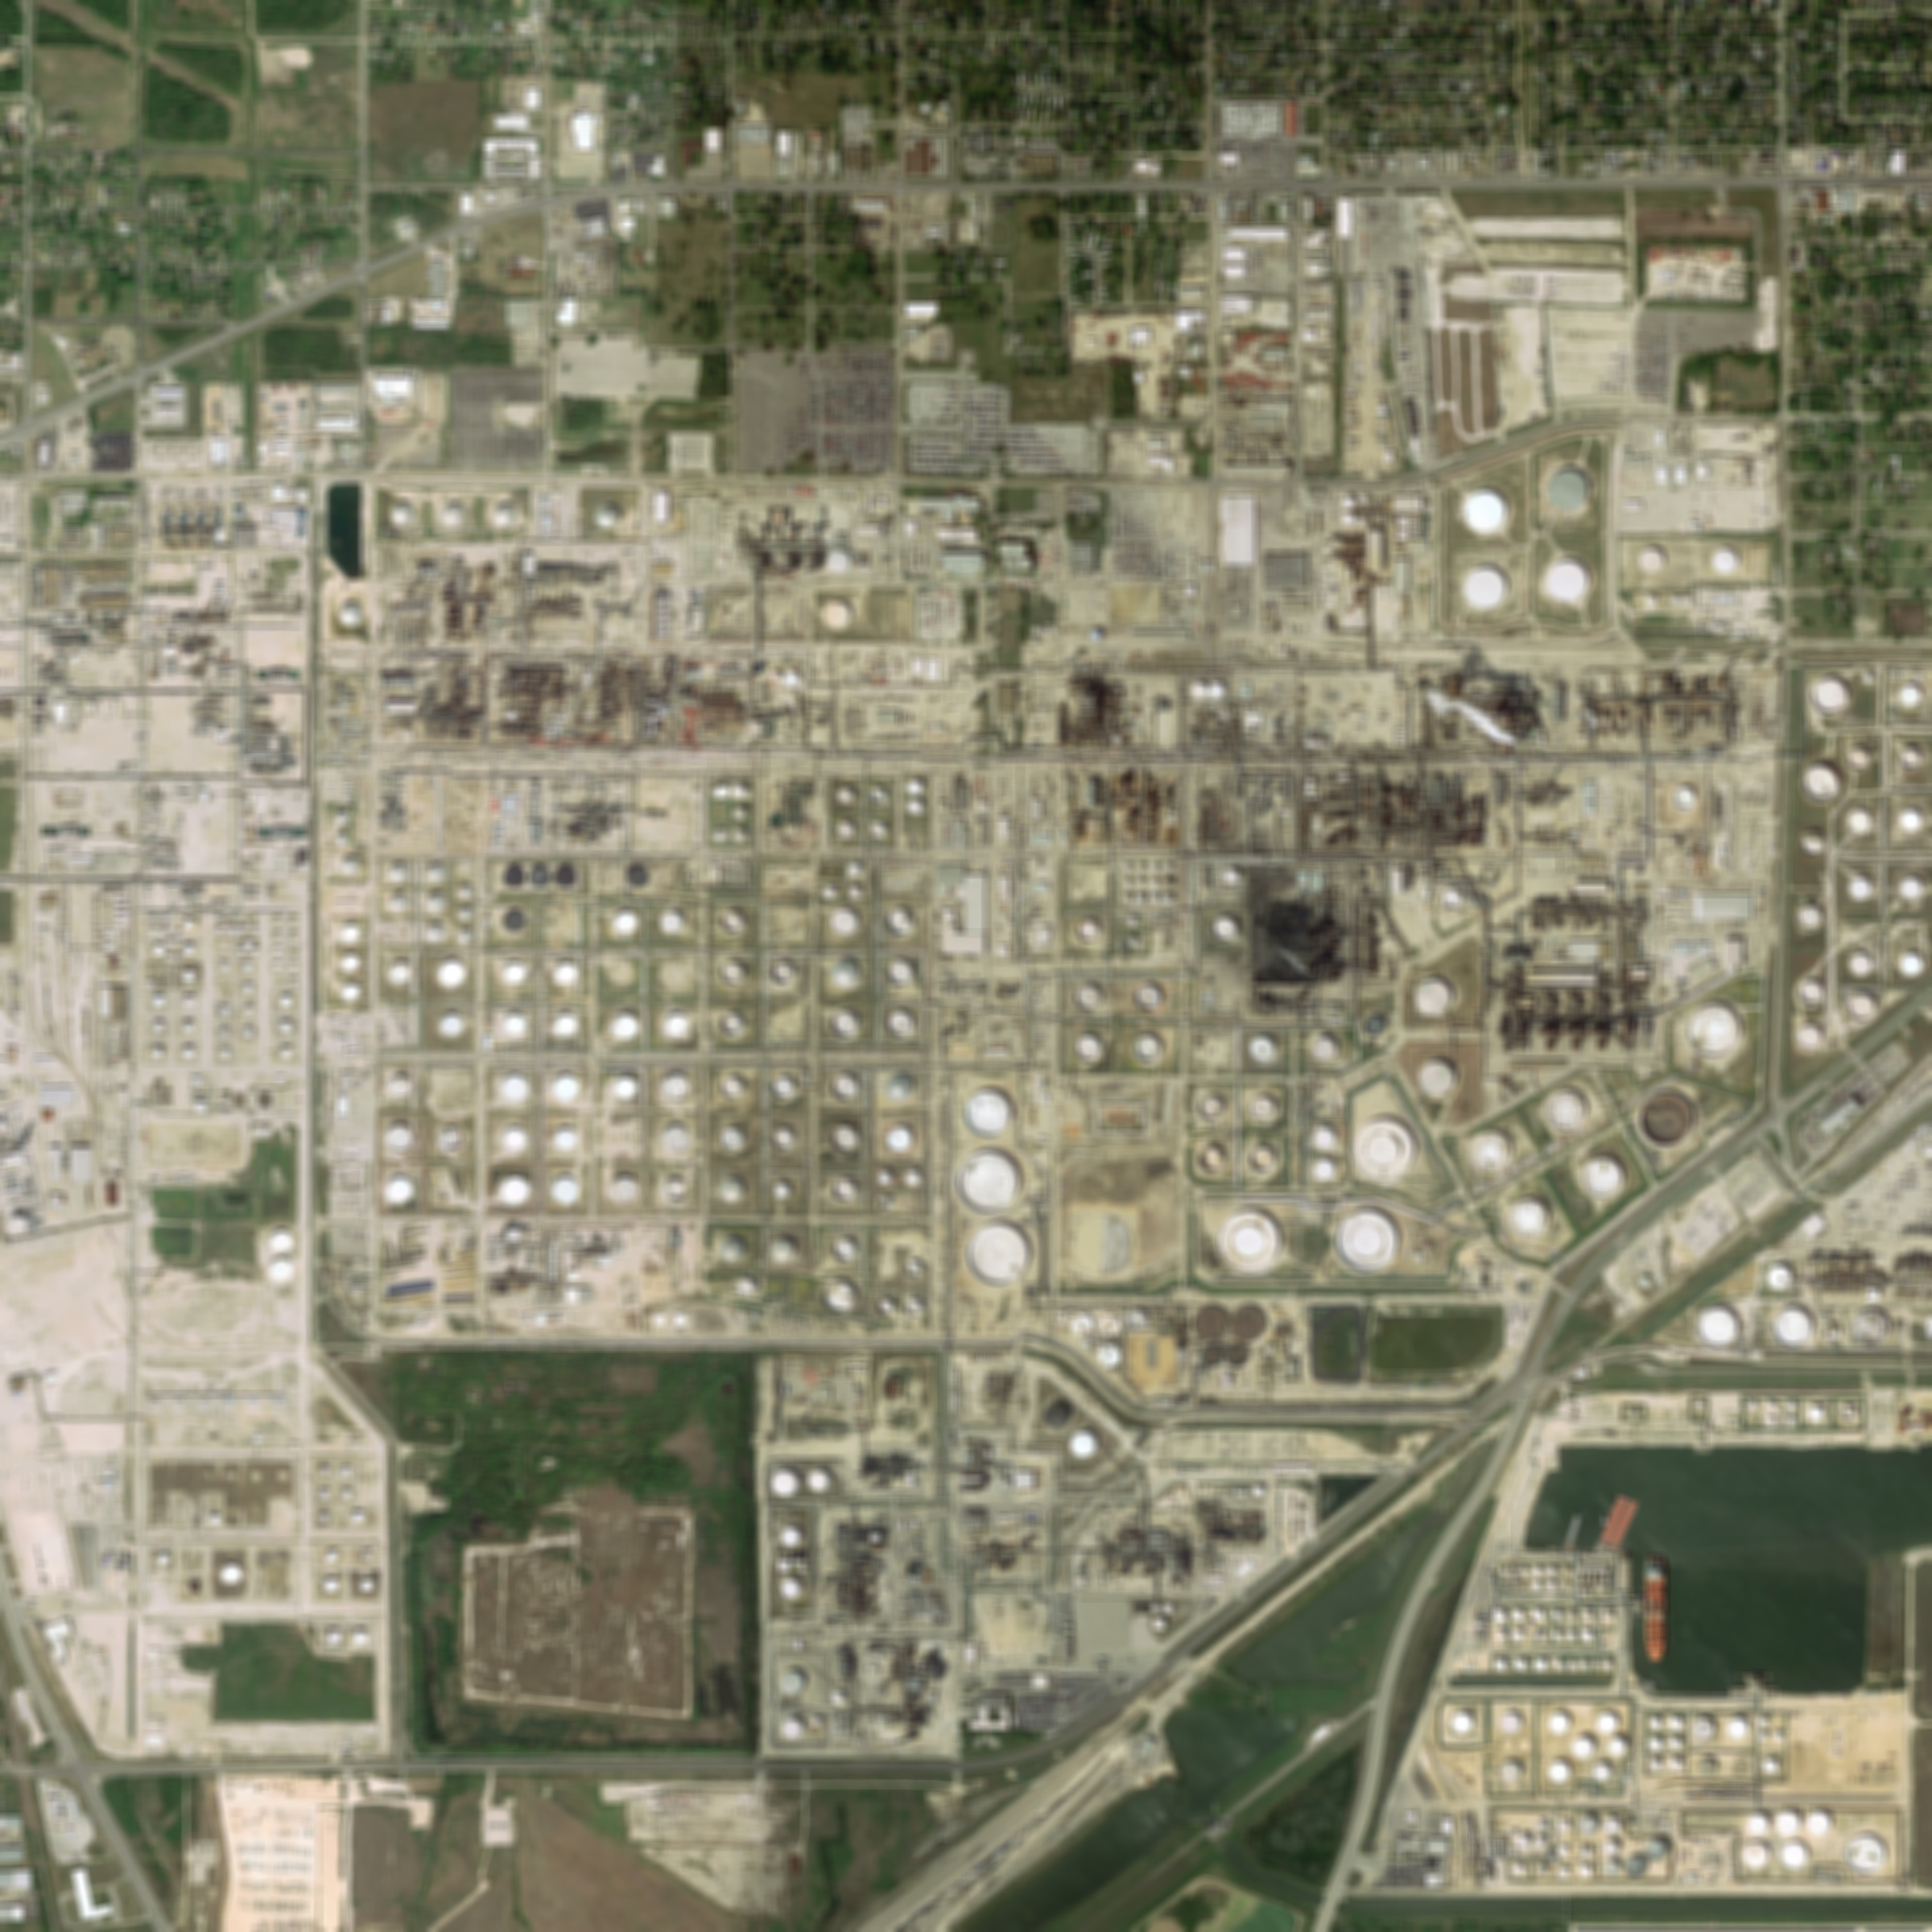
\includegraphics[width=0.25\textwidth]{images/smooth-filter/img1_avg.png}
\caption{Imagen industrial original y transformaciones mediante filtros de media y gaussiano. $K=25$.}
\label{fig:filtro_suavizado_industrial}
\end{figure}

\begin{figure}[h!]
\centering
\includegraphics[width=0.25\textwidth]{images/smooth-filter/img2_original.png}
\includegraphics[width=0.25\textwidth]{images/smooth-filter/img2_gaussian.png}
\includegraphics[width=0.25\textwidth]{images/smooth-filter/img2_avg.png}
\caption{Imagen médica original y transformaciones mediante filtros de media y gaussiano. $K=7$.}
\label{fig:filtro_suavizado_medico}
\end{figure}

Como se puede observar en el caso de las imágenes industriales, la aplicación del filtro de suavizado afecta notablemente a las componentes estructurales de la imagen. Especialmente en el caso del filtro de media, se aprecia una supresión agresiva de los bordes presentes. 

Para el caso de la imagen médica, se observa cómo pequeños elementos presentes en la imagen original, como los alvéolos pulmonares u otros componentes fibrosos de menor tamaño, desaparecen completamente, dejando a la vista órganos más relevantes y enfocando la imagen en estructuras de mayor escala.

Respecto a las métricas obtenidas tras las transformaciones, se muestran a continuación:

\begin{table}[h]
\centering
\caption{Métricas cuantitativas sobre las transformaciones aplicadas a ambas imágenes.}
\label{tab:metricas-suavizado}
\begin{tabular}{lcccc}
\hline
\textbf{Configuración} & \textbf{PSNR} & \textbf{SSIM} & \textbf{Entropy} & \textbf{EPI} \\
\hline
$Industrial_{avg}$   & 19.45 & 0.35 & 7.41 & 0.00 \\
$Industrial_{gauss}$ & 21.55 & 0.47 & 7.48 & 0.00 \\
$Medical_{avg}$      & 34.40 & 0.92 & 7.43 & 0.03 \\
$Medical_{gauss}$    & 37.79 & 0.96 & 7.42 & 0.22 \\
\hline
\end{tabular}
\end{table}

A continuación se comentan las métricas expuestas en la Tabla \ref{tab:metricas-suavizado}:

\begin{itemize}
    \item \textbf{PSNR}: El filtrado gaussiano presenta valores de PSNR superiores al filtrado promedio, lo que indica una menor distorsión píxel a píxel respecto a la imagen original.
    \item \textbf{SSIM}: El filtro gaussiano conserva mejor la estructura global de la imagen, especialmente en la imagen médica, donde se alcanzan valores de SSIM cercanos a 1.
    \item \textbf{Entropía}: La entropía se mantiene prácticamente constante tras el suavizado, lo que indica que no se produce una pérdida significativa de información global.
    \item \textbf{EPI}: El suavizado reduce de forma notable la preservación de bordes, siendo el filtro gaussiano claramente superior al filtro promedio, especialmente en la imagen médica.
\end{itemize}

\subsubsection{Realce de bordes}
En esta sección se presenta la aplicación de filtros de realce de bordes sobre imágenes seleccionadas de los datasets Open-I, Science Source y EOSDA LandViewer. Se han empleado los filtros Prewitt y Canny, dado que el filtro de Prewitt presenta un comportamiento muy similar al de Sobel y permite reducir la redundancia en el análisis, mientras que Canny se considera un detector de bordes más completo y robusto, lo que facilita la comparación de su comportamiento frente a distintos tipos de imágenes.

Para el estudio se han utilizado tres imágenes de naturaleza diferente: una imagen industrial, una radiografía de tórax y una imagen satelital. La imagen industrial se ha seleccionado con el objetivo de analizar la eficacia de los filtros en un escenario con una elevada densidad de bordes y estructuras geométricas bien definidas. Asimismo, se ha incluido una imagen de rayos X del tórax para evaluar la capacidad de los filtros para realzar de forma más nítida las estructuras óseas del cuerpo humano, caracterizadas por transiciones de intensidad más suaves y bordes menos definidos.

Por último, se ha añadido una imagen satelital correspondiente a un barrio residencial con el fin de comprobar si los filtros son capaces de realzar las distintas calles y elementos urbanos del núcleo. Dado que esta imagen presenta una resolución significativamente inferior al resto, ha sido necesario aplicar un reescalado previo con un factor $\times4$ mediante interpolación, ya que, en su tamaño original, los detalles resultaban imperceptibles y la aplicación de los filtros no producía resultados adecuados.

\begin{figure}[H]
\centering
\includegraphics[width=0.85\textwidth]{images/satelite_prewitt_canny.png}
\caption{Imagen industrial original y transformaciones mediante filtros de Prewitt y Canny.}
\label{fig:filtro_borde_industrial}
\end{figure}

\begin{figure}[H]
\centering
\includegraphics[width=0.85\textwidth]{images/rx_prewitt_canny.png}
\caption{Imagen médica original y transformaciones mediante filtros de Prewitt y Canny.}
\label{fig:filtro_borde_medico}
\end{figure}

\begin{figure}[H]
\centering
\includegraphics[width=0.85\textwidth]{images/res_prewitt_canny.png}
\caption{Imagen satelital original y transformaciones mediante filtros de Prewitt y Canny.}
\label{fig:filtro_borde_satelital}
\end{figure}

Como se puede observar en la Figura~\ref{fig:filtro_borde_industrial}, la aplicación del filtro de Canny en la imagen satelital produce un realce considerable de los bordes correspondientes a los caminos y a las estructuras de mayor tamaño. Este comportamiento permite identificar con claridad las principales infraestructuras presentes en la escena. No obstante, el resultado muestra un oscurecimiento general de la imagen y la pérdida de ciertos detalles asociados a edificios o estructuras de menor tamaño. Por el contrario, la imagen procesada con el filtro Prewitt no presenta un realce significativo de los bordes y, en términos generales, empeora la visualización con respecto a la imagen original, dificultando la identificación de las estructuras de interés.

En el caso de la Figura~\ref{fig:filtro_borde_medico}, se observa un comportamiento opuesto. El filtro Prewitt permite distinguir de manera más clara las estructuras óseas de la caja torácica, así como los huesos del hombro y del brazo, manteniendo una mayor continuidad en los contornos. En cambio, el filtro Canny genera únicamente algunas líneas inconexas correspondientes a los huesos, lo que impide apreciar las distintas estructuras óseas de forma completa y dificulta su interpretación visual.

Por último, en la Figura~\ref{fig:filtro_borde_satelital}, al igual que en la Figura~\ref{fig:filtro_borde_medico} el filtro Prewitt distingue mejor los diferentes bordes de las calles incluso ha reconocido alguna vivienda o estructura grande. El filtro Canny en este caso no ha sido capaz de distinguir nada claramente, salvo un par de viviendas pero no hay ninguna estructura definida en la transformacion. Ambas cosas pueden ser debidas a la mala calidad de la imagen y debido a ello los filtros se comporten de manera diferente.

A continuación se muestran las métricas obtenidas en las imagenes:

\begin{table}[h]
\centering
\caption{Métricas cuantitativas sobre las transformaciones aplicadas a ambas imágenes.}
\label{tab:metricas-edge}
\begin{tabular}{lcccc}
\hline
\textbf{Configuración} & \textbf{PSNR} & \textbf{SSIM} & \textbf{Entropy} & \textbf{EPI} \\
\hline
$Industrial_{prew}$   & 8.09 & 0.04 & 11.15 & 1.84 \\
$Industrial_{can}$ & 5.82 & 0.00 & 0.50 & 2.35 \\
$Medical_{prew}$      & 6.66 & 0.14 & 9.06 & 1.77 \\
$Medical_{can}$    & 5.56 & 0.04 & 0.13 & 1.92 \\
$satelital{prew}$      & 11.55 & 0.10 & 10.84 & 1.45 \\
$satelital{can}$    & 6.52 & 0.01 & 0.84 & 2.83 \\
\hline
\end{tabular}
\end{table}

\begin{itemize}
    \item \textbf{PSNR}: Los valores de PSNR obtenidos son bajos en ambos filtros, lo que indica una modificación significativa de la imagen original. El filtro Prewitt presenta, en general, valores de PSNR superiores a los del filtro Canny, reflejando una transformación menos agresiva de la imagen.
    
    \item \textbf{SSIM}: El filtro Prewitt tiende a conservar mejor la estructura global de la imagen, alcanzando valores de SSIM superiores a los obtenidos con Canny. En contraste, el filtro Canny muestra valores de SSIM muy reducidos, debido a su carácter selectivo y a la eliminación de gran parte de la información estructural.
    
    \item \textbf{Entropía}: La entropía es considerablemente mayor en las imágenes procesadas con Prewitt, lo que indica la conservación de una mayor cantidad de información y detalle. Por el contrario, el filtro Canny produce valores de entropía muy bajos, reflejando una simplificación notable de la imagen al retener únicamente los bordes más relevantes.
    
    \item \textbf{EPI}: El filtro Canny presenta valores de EPI más elevados, lo que indica una detección más intensa de gradientes fuertes. Sin embargo, este comportamiento no implica necesariamente una mejor preservación estructural. El filtro Prewitt, aunque obtiene valores de EPI inferiores, mantiene una mayor continuidad de los bordes y una representación más fiel de las estructuras originales.
\end{itemize}

\subsection{Filtros Morfológicos}
\label{sec:filtros_morf}

\subsubsection{Dilatación}
\label{sec:dil}

En esta sección se presenta el efecto del filtro morfológico de dilatación sobre una imagen seleccionada del dataset \textit{EOSDA LandViewer}. 
Este filtro, como ya se ha comentado antes, tiene como principal objetivo expandir las áreas de interés, conectando componentes cercanos y rellenando huecos en las estructuras presentes en la imagen. 
A través de este proceso, las zonas de interés (en este caso, las áreas de agua) se amplían, mejorando su visibilidad y su posible detección.

Para esta imagen, el elemento estructurante utilizado es de tamaño \( 3 \times 3 \), lo que significa que se está ampliando cada píxel en un vecindario de 3 píxeles alrededor del píxel central. 
Cuanto mayor sea el tamaño del kernel, más se expandirán las áreas de interés. Además, se ha utilizado una sola iteración que controla cuántas veces se aplica la operación de dilatación a la imagen. 
Aumentar el número de iteraciones ampliará aún más las áreas de interés, lo que podría ser útil para imágenes más fragmentadas, aunque tras realizar diferentes pruebas se ha comprobado que sobre esta imagen no era necesario.

Se decidió aplicar la dilatación exclusivamente sobre el canal azul de la imagen, para resaltar y expandir las áreas de agua sin afectar los otros canales de color (rojo y verde), los cuales no contienen tanta información relevante para nuestro objetivo.
En todo caso, con intención de mostrar la información completa también se mostrará el filtro aplicado a todos los canales.

En la siguiente figura \ref{fig:filtros_dilatacion}, se muestran los resultados tras aplicar la dilatación a la imagen en tres casos diferentes: la imagen original (izquierda), la dilatación aplicada sin diferenciar canales (en medio) y la dilatación aplicada únicamente al canal azul (derecha).

\begin{figure}[h!]
\centering
\includegraphics[width=0.25\textwidth]{images/fdilatacionorigin.png}
\includegraphics[width=0.25\textwidth]{images/fdilatacionNormal.png}
\includegraphics[width=0.25\textwidth]{images/fdilatacion-result.png}
\caption{Ejemplo de imagen procesada con el filtro de dilatación en tres condiciones.}
\label{fig:filtros_dilatacion}
\end{figure}

La imagen original muestra las zonas de agua destacando menos, con algunas áreas fragmentadas y menos definidas. 
Si se aplicara la dilatación sobre todos los canales de color (rojo, verde y azul) de la imagen en lugar de solo al canal azul, como se puede observar en la Figura \ref{fig:filtros_dilatacion}, el filtro afectaría a las áreas de color de manera más general, lo que podría no ser ideal si el objetivo principal es resaltar únicamente las zonas de agua.
De hecho, al aplicar dilatación sobre los tres canales, el filtro altera otras áreas de la imagen que no son de interés, afectando negativamente a la definición de estas áreas.

Por otro lado, al implementar el filtro solo al canal azul, se observa una expansión más clara de las zonas objetivo, mejorando su visibilidad y conectividad sin afectar otras áreas de la imagen, demostrando ser un enfoque más eficiente con el objetivo asignado en este caso.

En términos de métricas cuantitativas sobre la imagen con el filtro aplicado solo al canal azul, se ha observado lo siguiente:

\begin{itemize}
    \item \textbf{PSNR}: 32.88. La imagen dilatada muestra una ligera disminución, indicando que la dilatación ha introducido ciertos cambios en la imagen, pero que son mínimos,
    Esto sugiere que la calidad de la imagen se conserva bastante bien.
    \item \textbf{SSIM}: 0.9918. El valor de SSIM es extremadamente alto, representando que la dilatación no ha alterado significativamente la estructura global de la imagen, aunque se ha mejorado la visibilidad de las áreas de agua.
    \item \textbf{Entropía}: 6.9063. La entropía disminuye ligeramente, lo que indica que la imagen se ha simplificado al expandir las áreas de agua y rellenar huecos, eliminando detalles pequeños en el proceso.
    \item \textbf{EPI}: 1.5542. Los valores de EPI son relativamente bajos, lo que sugiere que la dilatación ha preservado los bordes más grandes de las zonas de agua, pero ha suavizado los bordes finos en las áreas dilatadas.
\end{itemize}


\subsubsection{Erosión}
\label{sec:er}

En esta segunda sección, se presenta el efecto del filtro morfológico de erosión sobre la imagen del dataset \textit{Open-i}. 
Este se ha aplicado bajo las mismas condiciones que la dilatación, con un valor de elemento estructurante (kernel de tamaño \(3 \times 3\)) y número de iteraciones (una iteración).

La siguiente figura muestra el resultado antes y después de aplicar la erosión a la imagen:

\begin{figure}[h!]
\centering
\includegraphics[width=0.35\textwidth]{images/fErosionOriginal.png}
\includegraphics[width=0.35\textwidth]{images/fErosionFinal.png}
\caption{Ejemplo de imagen procesada con el filtro de erosión morfológica.}
\end{figure}

La imagen original muestra todas las estructuras, incluidas las pequeñas imperfecciones y detalles que no son relevantes para el análisis de las zonas óseas.

En este caso, se observa un cambio sutil en la imagen tras aplicar la erosión, donde los detalles pequeños han sido eliminados simplificando la imagen. 
Esto hace que las áreas más grandes, como las costillas y los pulmones, sean más visibles y fáciles de identificar.

En términos de métricas cuantitativas, se ha observado lo siguiente:

\begin{itemize}
    \item \textbf{PSNR}: 34.87. La imagen dilatada muestra una mínima disminución en el valor de PSNR, lo que indica que la erosión ha introducido ciertos cambios en la imagen sin alterar la calidad general.
    \item \textbf{SSIM}: 0.9337. El valor de SSIM es relativamente alto, lo que sugiere que la erosión no ha alterado significativamente la estructura global de la imagen incluso habiendo suavizado los detalles más pequeños.
    \item \textbf{Entropía}: 7.7583. La entropía ha aumentado, lo que indica que la imagen se ha simplificado al eliminar detalles pequeños y suavizar áreas irrelevantes, facilitando la visualización de las estructuras principales, como los huesos.
    \item \textbf{EPI}: 3.3505. Los valores de EPI muestran una ligera disminución, lo que sugiere que la erosión ha suavizado los bordes finos, pero ha preservado la estructura general de la imagen, mejorando la conectividad entre las áreas relevantes.
\end{itemize}

Tras este análisis, se puede afirmar que el filtro de erosión resulta ser una herramienta útil para analizar las estructuras principales en la imagen, como los huesos, quitando detalles irrelevantes. 
Aunque los cambios no son grandes, se aprecia cómo la erosión mejora la visibilidad de las zonas importantes, como las costillas y los pulmones, al reducir el ruido en las áreas más oscuras. 

\subsubsection{Apertura}
\label{sec:apt}

A continuación, se muestra cómo afecta el filtro morfológico de apertura a las imágenes seleccionadas. Para cada imagen se muestran los cambios introducidos sobre la estructura y los detalles, permitiendo observar de manera directa cómo esta técnica 
modifica la geometría de los objetos. Además, se incluyen métricas que cuantifican el impacto del filtro en términos de calidad visual y preservación de estructuras relevantes.

\begin{figure}[h!]
    \centering
    \includegraphics[width=0.6\textwidth]{images/fapertura.png}
    \caption{Ejemplo de imagen procesada con el filtro de apertura morfológica.}
    \label{fig:apertura}
\end{figure}

\begin{itemize}
    \item \textbf{Austin\_2973:} Se observa una reducción de la textura detallada de los árboles y de los caminos estrechos, lo que indica que se ha suavizado la imagen y se han simplificado las estructuras finas.

    \item \textbf{CXR2046:} La imagen presenta cambios más sutiles. El filtro suaviza ligeramente el ruido de la placa, pero conserva casi perfectamente la estructura ósea y pulmonar.

    \item \textbf{PermanentCrop\_1643:} Debido a la baja resolución y al carácter pixelado de la imagen, el filtro elimina detalles pequeños y unifica bloques de color, generando una apariencia más plana y uniforme.
\end{itemize}

\medskip
Las métricas cuantitativas de estas observaciones indican lo siguiente:

\begin{itemize}
    \item \textbf{PSNR:} La radiografía alcanza un valor de 42.95, lo que indica que la imagen transformada es casi idéntica que la imagen original. Las imágenes de Austin y PermanentCrop presentan valores más bajos, en torno a 25-28, lo que refleja una mayor pérdida de información estructural.
    \item \textbf{SSIM:} La radiografía mantiene un valor cercano a 1 (0.994), mientras que PermanentCrop y Austin bajan a 0.826 y 0.776 respectivamente, mostrando que la apertura afecta más a la composición de estas últimas.
    \item \textbf{Entropía:} Disminuye en todos los casos, lo que indica que la apertura simplifica la imagen al eliminar detalles pequeños y ruido.
    \item \textbf{EPI:} Los valores se reducen notablemente, especialmente en PermanentCrop (cercano a 0), confirmando que los bordes finos son suavizados o eliminados.
\end{itemize}

En la imagen médica, el filtro de apertura es bastante conservador, reduciendo el ruido sin afectar la estructura principal, mientras que en las imágenes satelitales y aéreas tiende a eliminar detalles pequeños, resaltando las formas y estructuras más grandes.

\subsubsection{Cierre}
\label{sec:cierr}

A continuación, se muestra cómo afecta el filtro morfológico de cierre a las imágenes seleccionadas. Para cada imagen se muestran los cambios introducidos sobre la estructura y los detalles, permitiendo observar de manera directa cómo esta técnica 
modifica la geometría de los objetos. Además, se incluyen métricas que cuantifican el impacto del filtro en términos de calidad visual y preservación de estructuras relevantes.

\begin{figure}[h!]
    \centering
    \includegraphics[width=0.6\textwidth]{images/fcierre.png}
    \caption{Ejemplo de imagen procesada con el filtro de cierre morfológica.}
    \label{fig:cierre}
\end{figure}

\begin{itemize}
    \item \textbf{Austin\_2973:} Las texturas finas, como las copas de los árboles, se suavizan, dando a la imagen un aspecto más uniforme.
    \item \textbf{CXR2046:} La imagen presenta gradientes suaves y pocos detalles oscuros aislados, por lo que el filtro apenas altera la estructura original.
    \item \textbf{PermanentCrop\_1643:} Se observa un suavizado en los bordes de las parcelas y una reducción del ruido granular en zonas oscuras, manteniendo la forma general de los objetos.
\end{itemize}

\medskip
Las métricas cuantitativas de estas observaciones indican lo siguiente:

\begin{itemize}
    \item \textbf{PSNR:} La radiografía alcanza un valor de 49.02, lo que indica que la imagen transformada es casi idéntica que la imagen original. En cambio, la imagen de Austin presenta un valor de 26.50 dB, lo que indica que la estructura de la imagen se ha modificado más.
    \item \textbf{SSIM:} La radiografía conserva un valor muy cercano a 1 (0.997), mientras que la imagen satelital desciende a 0.80, indicando que se han suavizado o perdido detalles finos.
    \item \textbf{Entropía:} Disminuye en todos los casos, lo que indica que el filtro reduce el ruido y la información visual, dejando las imágenes más uniformes.
    \item \textbf{EPI:} Los valores se reducen bastante, especialmente en la imagen Austin, lo que confirma que los bordes nítidos se suavizan o redondean al cerrar los pequeños huecos.
\end{itemize}

En la imagen médica, el filtro de cierre tiene un efecto mínimo, suavizando ligeramente pequeñas zonas oscuras sin alterar la estructura principal, mientras que en las imágenes satelitales y aéreas tiende a rellenar huecos y suavizar detalles finos, dando como resultado áreas más uniformes y compactas.

\section{Discusión}
\label{sec:discusion}

En conjunto, los resultados muestran que el filtrado espacial no debe ser interpretado como un paso de mejora universal, sino como una transformación con efectos específicos que dependen del objetivo (reducción de ruido, preservación estructural, o mejora de bordes) y las características de la escena (textura, contraste, y escala). En este sentido, el principal hallazgo es la existencia de un \textit{trade-off} entre el suavizado y la preservación de los detalles: las técnicas mas agresivas en reducir la variabilidad local tienden a degradar los bordes y microestructuras, mientras que otras aproximaciones mas conservativas son mejores preservando geometría pero dejan mas residuo de ruido o textura.

Las métricas cuantitativas respaldan esta lectura, pero deben ser interpretadas en relación con el propósito del procesado. Métricas como PNSR y SSIM premian la similitud con la imagen original, lo cual es útil para la estimación global de la distorsión, aunque no necesariamente refleja una mejora funcional cuando el objetivo es facilitar tareas posteriores (por ejemplo, segmentación o detección). En cambio, indicadores relacionados con los bordes y los componentes estructurales proveen de una señal complementaria sobre pérdida o preservación de contornos, reforzando que la calidad "optima" no es absoluta, si no que depende del criterio de uso. 

De forma paralela, el análisis muestra que la parametrización es determinante: el tamaño del kernel, el elemento estructurante y los umbrales de detección condicionan tanto o mas que el método elegido. Por lo tanto, la elección de los parámetros debe ser consistente con la escala de los objetos de interés: parámetros grandes favorecen regularización y conectividad, pero pueden borrar información fina; parámetros pequeños preservan el detalle, pero pueden ser insuficientes para estabilizar el ruido o consolidar regiones. 

Finalmente, el conjunto de técnicas consideradas sugiere una recomendación general: conviene alinear el filtrado con una intención explicita y, cuando sea posible, evaluar su impacto desde un punto de vista orientado a tareas posteriores. En otras palabras, en vez de buscar el "mejor filtro" en términos generales, resulta más consistente seleccionar una combinación de operadores y parámetros que optimice el equilibrio relevante para el problema, dejando las conclusiones finales como síntesis de dichas decisiones y sus implicaciones. 

\section{Conclusiones}
\label{sec:conclusiones}

Este trabajo ha analizado el comportamiento practico de un conjunto representativo de \textit{filtros espaciales} y \textit{operaciones morfologicas} cuando son aplicadas a imágenes reales de tres dominios heterogéneos (medico, industrial y satelital). El objetivo principal era caracterizar como cada técnica modificaba la información visual, como preservaba las estructuras relevantes y como la interpretabilidad cambia en función del método y de su parametrización. Para realizar una comparación robusta, la evaluación combino inspecciones cualitativas con indicadores cuantitativos, incluyendo PNSR, SSIM, entropía e indice de preservación de bordes (EPI).

En general, los resultados confirman que no hay un único operador que pueda ser considerado universalmente optimo. En cambio, el rendimiento del filtro se ve altamente condicionado por (i) el contenido de la imagen (textura, distribución de contrastes, y escala del objeto), (ii) el propósito (eliminar ruido, enfatizar bordes, o consolidación estructural), y (iii) los parámetros seleccionados (tamaño de kernel, elemento estructural, y umbrales). En particular, los filtros de suavizado presentan constantemente un \textit{trade-off}: el incremento de la atenuación de ruido incrementa el riesgo de bordes borrosos y de atenuar detalles finos. Adicionalmente, operaciones de realce de bordes mejoran la saliencia de los límites pero pueden amplificar ruidos y generar artefactos cuando la escena contenga texturas de alta frecuencia o cuando el suavizado previo sea insuficiente. 

Los operadores morfológicos demostraron ser especialmente eficaces para controlar la conectividad y la geometría en regiones binarizadas o de alto contraste. La erosión y la apertura tienden a eliminar pequeños componentes brillantes y protuberancias delgadas, lo cual es beneficioso para eliminar artefactos aislados pero también pueden eliminar microcaracteristicas clínicas o estructuralmente relevantes. La dilatación y el cierre generalmente consolidan regiones fragmentadas y rellenan pequeños huecos, mejorando la continuidad de la región a costa del engrosamiento de los límites y la posible fusión de estructuras cercanas. Estos efectos se han ido mostrando constantemente en las métricas cuantitativas de la misma manera que con los filtros espaciales. 

Desde el punto de vista de aplicación de las técnicas, la principal implicación metodológica es que la selección del filtro debe ser formulada como una decisión de diseño orientada a objetivos, en lugar de como un paso de mejora genérico. Los resultados mas fiables se obtuvieron cuando la elección de parámetros estaba alineada con la escala espacial de las estructuras. Consecuentemente, se recomienda (i) definir explícitamente el objetivo final (por ejemplo, preparación para segmentación, localización de bordes o regularización de regiones), (ii) restringir los rangos de parámetros en función del tamaño esperado del objeto, y (iii) evaluar los resultados con una combinación de métricas perceptuales y estructurales, evitando depender exclusivamente de PNSR/SSIM cuando la transformación es intencionalmente no conservadora. 

Finalmente, este estudio presenta varias lineas naturales para trabajos futuros. Primero, la extensión del dataset y la implementación de modelos de ruido (por ejemplo, speckle, Poisson) reforzarían la generalización en diferentes condiciones de adquisición. En segundo lugar, evaluar el rendimiento con métricas a nivel de tarea (por ejemplo, precisión de segmentación, precisión/recuperación de la detección) proporcionaría una noción de mejora mas operativa que la simple similitud. En tercer lugar, la optimización sistemática de la parametrización podría formalizar el proceso de selección y reducir la subjetividad. Estas ampliaciones consolidarían aún más la conclusión central de este proyecto: un filtrado de imágenes eficaz depende intrínsecamente del contexto y debe ajustarse a las características de la imagen y al objetivo analítico previsto.

\section{Distribución del trabajo}
\label{sec:distribuciontrabajo}

\begin{table}[H]
\centering
\caption{Organización del trabajo en grupo.}
\label{tab:dist-work}
\begin{tabular}{lcccc}
\hline
\textbf{Apartado de la memoria} & \textbf{Responsables} \\
\hline
Resumen   & Nuria, León, Pau y Álvaro \\
Introducción & Nuria, León, Pau y Álvaro \\
Material y métodos  & Nuria, León, Pau y Álvaro \\
Resultados y métricas    & Nuria, León, Pau y Álvaro \\
Discusión  & Nuria, León, Pau y Álvaro \\
Conclusiones  & Nuria, León, Pau y Álvaro \\
\hline
\end{tabular}
\end{table}

\section{Declaración de la IA}
\label{sec:declaracionia}
A lo largo del desarrollo de esta propuesta se ha utilizado la IA como una herramienta de apoyo, con el principal objetivo de resolver dudas, obtener orientación estructural y conceptual y para mejorar la redacción de algunos 
apartados. Es importante destacar que no se ha utilizado la IA para desarrollar el proyecto en su totalidad, sino como un recurso complementario. La mayoría de las respuestas ofrecidas presentan imprecisiones o información no válida, 
por lo ha sido necesario contrastar la respuesta con fuentes fiables. 

\printbibliography

\end{document}